\ifx\all\undefined
\documentclass[spanish,a4paper,11pt]{book}

%----------------------------
\usepackage[spanish,es-noquoting,es-tabla]{babel}
\usepackage[latin1]{inputenc}
\usepackage[T1]{fontenc}
%----------------------------
\usepackage{graphicx}
\usepackage[citecolor=black, urlcolor=black, linkcolor=black, colorlinks=true, bookmarksopen=true]{hyperref}
\usepackage{cleveref}
\usepackage{float}
\usepackage{enumitem}
% \usepackage[toc]{glossaries} %xindy
% \makeglossaries
%----------------------------
\usepackage{amsmath}

\makeatletter
\newcommand*{\bdiv}{%
  \nonscript\mskip-\medmuskip\mkern5mu%
  \mathbin{\operator@font div}\penalty900\mkern5mu%
  \nonscript\mskip-\medmuskip
}
\makeatother

\usepackage[]{geometry}
\usepackage{tikz}
\usepackage[simplified]{pgf-umlcd}
\usepackage{pgf-umlsd}
%----------------------------
%CODE:
\usepackage[procnames]{listings}
\usepackage{color}
\usepackage{tablefootnote}

\definecolor{keywords}{RGB}{255,0,90}
\definecolor{comments}{RGB}{0,0,113}
\definecolor{red}{RGB}{160,0,0}
\definecolor{green}{RGB}{0,90,0}
\definecolor{gray}{RGB}{190,190,190}
\definecolor{mauve}{RGB}{160,126,175}

\crefname{table}{\spanishtablename}{\spanishtablename}
\crefname{listing}{código fuente}{códigos fuente}

\lstset{language=Python, 
        basicstyle=\ttfamily\small, 
        keywordstyle=\color{keywords},
        commentstyle=\color{comments},
        stringstyle=\color{red},
        breaklines=true, 
        showstringspaces=false,
        identifierstyle=\color{green},
        tabsize=2,
        procnamekeys={def,class}
        numbers=left,
        frame=single,
        numbers=left,
        numbersep=5pt,
        numberstyle=\tiny
}

% \lstset{language=C++,
% basicstyle=\footnotesize\sffamily\color{black},
% commentstyle=\color{gray},
% frame=single,
% numbers=left,
% numbersep=5pt,
% numberstyle=\tiny\color{gray},
% keywordstyle=\color{green},
% showspaces=false,
% showstringspaces=false,
% stringstyle=\color{orange},
% tabsize=2
% }

% \lstset{ %
%   backgroundcolor=\color{white},   % choose the background color; you must add \usepackage{color} or \usepackage{xcolor}
%   basicstyle=\footnotesize,        % the size of the fonts that are used for the code
%   breakatwhitespace=false,         % sets if automatic breaks should only happen at whitespace
%   breaklines=true,                 % sets automatic line breaking
%   captionpos=b,                    % sets the caption-position to bottom
%   commentstyle=\color{green},    % comment style
%   %deletekeywords={...},            % if you want to delete keywords from the given language
%   escapeinside={\%*}{*)},          % if you want to add LaTeX within your code
%   extendedchars=true,              % lets you use non-ASCII characters; for 8-bits encodings only, does not work with UTF-8
%   frame=single,                    % adds a frame around the code
%   keepspaces=true,                 % keeps spaces in text, useful for keeping indentation of code (possibly needs columns=flexible)
%   keywordstyle=\color{blue},       % keyword style
%   language=Octave,                 % the language of the code
%   morekeywords={},            % if you want to add more keywords to the set
%   numbers=left,                    % where to put the line-numbers; possible values are (none, left, right)
%   numbersep=5pt,                   % how far the line-numbers are from the code
%   numberstyle=\tiny\color{gray}, % the style that is used for the line-numbers
%   rulecolor=\color{black},         % if not set, the frame-color may be changed on line-breaks within not-black text (e.g. comments (green here))
%   showspaces=false,                % show spaces everywhere adding particular underscores; it overrides 'showstringspaces'
%   showstringspaces=false,          % underline spaces within strings only
%   showtabs=false,                  % show tabs within strings adding particular underscores
%   stepnumber=2,                    % the step between two line-numbers. If it's 1, each line will be numbered
%   stringstyle=\color{mauve},     % string literal style
%   tabsize=2,                       % sets default tabsize to 2 spaces
%   title=\lstname                   % show the filename of files included with \lstinputlisting; also try caption instead of title
% }

\crefname{lstlisting}{fragmento}{fragmentos}
\Crefname{lstlisting}{Fragmento}{Fragmentos}
\renewcommand\lstlistingname{Fragmento}
\renewcommand\lstlistlistingname{Fragmentos}
\def\lstlistingautorefname{Frag.}

\usepackage{pdfpages}
%----------------------------
\newcommand{\ie}[0]{{\em i.e.,}}
\newcommand{\eg}[0]{{\em e.g.}}
\newcommand{\etal}[0]{{\em et al.}}
\newcommand{\etc}[0]{{\em etc.}}
\newcommand{\sdt}[0]{\textbf{SDT}}
\newcommand{\pat}[0]{\textbf{PAT}}
\newcommand{\cat}[0]{\textbf{CAT}}
\newcommand{\pmt}[0]{\textbf{PMT}}
\newcommand{\pid}[0]{\textbf{PID}}
\newcommand{\pes}[0]{\textbf{PES}}
\newcommand{\nit}[0]{\textbf{NIT}}


\renewenvironment{package}[2][\umlcdPackageTitle]{
\edef\umlcdPackageTitle{#2}
\def\umlcdPackageFit{}
\def\umlcdPackageName{#1}
}{
  \begin{pgfonlayer}{background}
  \node[umlcd style, draw, inner sep=0.5cm, fit = \umlcdPackageFit] (\umlcdPackageName) {};
  \node[umlcd style, draw, outer ysep=-0.5, anchor=south west] (\umlcdPackageName caption) at
  (\umlcdPackageName.north west) {\umlcdPackageTitle};
  \end{pgfonlayer}
}
\begin{document}
\fi

\newpage

\chapter{Merengue merengue} \label{App:AppendixA}

Saracatunga

\begin{figure}[h!]
	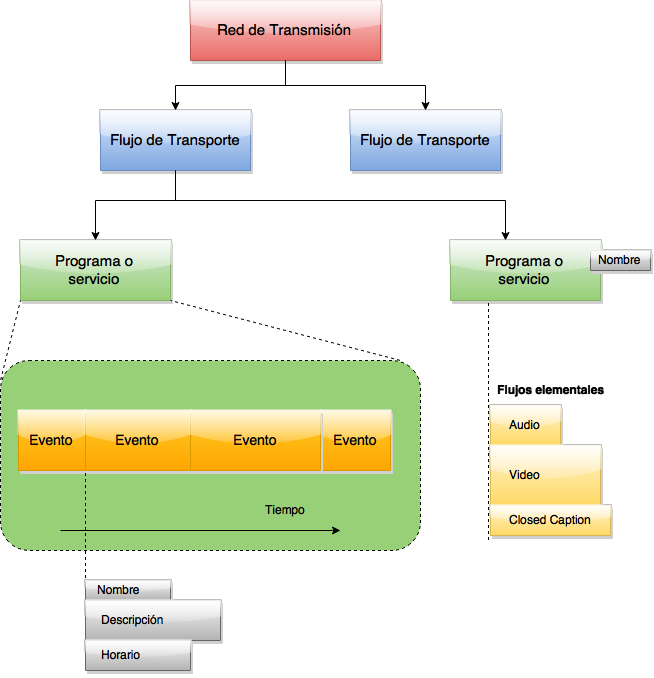
\includegraphics[width=12cm]{imgs/mpeg_structure.png}
	\caption{Diagrama de composici�n de un flujo de transporte} 
	\centering 
\end{figure}

\begin{itemize}
\item \textbf{Red de transmisi�n o \emph{network}:} Uno o m�s flujos de transporte emitidos por una misma entidad.
\item \textbf{Flujo de transporte:} Un flujo \textbf{MPEG-2} que lleva uno o m�s servicios.
\item \textbf{Servicio:} Alg�n contenido que puede consumir un receptor, \eg\ un canal de televisi�n, un canal de radio o un servicio de ingenier�a. 
\item \textbf{Evento:} Un programa de televisi�n. Dos eventos de un mismo servicio s�lo est�n diferenciados por el momento en que se est� sintonizando un servicio espec�fico.
\item \textbf{Flujo elemental o \emph{elementary stream}:} Un evento est� compuesto por uno o m�s flujos elementales. A su vez, puede contener m�s de un flujo del mismo tipo. \eg\ un show de televisi�n puede estar emiti�ndose en varios idiomas al mismo tiempo (un audio en ingl�s y otro en espa�ol). Los flujos elementales requieren de la mayor parte del ancho de banda de un flujo de transporte.
\end{itemize}

\subsubsection{Ejemplo de transport stream}

Continuando con el ejemplo introducido previamente transmitido por la frecuencia 527 Mhz, se puede ahondar en el an�lisis a trav�s de la jerarqu�a anterior:

\begin{itemize}
\item \textbf{Red de transmisi�n o \emph{network}:} El nombre de la red de transmisi�n es ``RTA C23'' que es administrada por Radio y Televisi�n Argentina S.E[TODO: Agregar cita]. 
\item \textbf{Flujo de transporte:} El flujo de transporte son los contenidos enviados por el canal f�sico 23 correspondiente a la frecuencia 527 Mhz.
\item \textbf{Servicios:} Presenta 3. TV P�blica HD, Tecn�polis y TV P�blica.
\item \textbf{Evento:} Son los distintos shows de cada canal. Por ejemplo, a las 14:00 horas del 5 de Junio comienza una emisi�n de ``Ciencia ahora''.
\item \textbf{Flujo elemental o \emph{elementary stream}:} Los flujos elementales pueden cambiar dependiendo del evento emitido en el momento. En el caso del fragmento utilizado, presenta 4 audios y 3 videos. Existen en el flujo de transporte otros \emph{elementary streams} que caen fuera del alcance de este informe.
\end{itemize}

\newpage
\chapter{Contribuci\'on y resultados obtenidos}

\newpage
\chapter{Temas de ap�ndice}

\begin{itemize}
\item Estructura del paquete de transport stream / Repasar el formato mpeg entero

\item Lista completa de las tablas de ISDB-Tb. Juntar con la de abajo.
\item Lista completa de los descriptores ISDB-Tb. Juntar con el de abajo
\item Lista de pids reservados, puede ir junto a lo de la tabla.

\item Comunicaci�n de threads en Wari
\item Descompresi�n de audio y video? 

\item Compilaci�n de Mara?
\item Construcci�n y utilizaci�n de herramientas en wari
\item OpenCaster?
\item DSM-CC explicado quiz� es demasiado.
\end{itemize}

\ifx\all\undefined
\end{document}
\fi



%%%%%%%%%%%%%%%%%%%%%%%%%%%%%%%%%%%%%%%%%%%%%%%%%%%%%%%%%%%%%%%%%%%%%%%%%%%%%%%%%%%%%%%%%%%%%%%%%%%%%%%%%%%%%%%%%%%%%
